\chapter{Fretha的测试}

\section{引言}
\ifshowtext

软件测试是确保软件质量和性能的重要环节。结合Fretha的应用实验,我们对软件的功能模块进行了测试,包括成像参数设置、数据导入导出、结果保存、软件性能和稳定性等方面。测试结果表明,Fretha软件在大部分情况下能够正常工作,但在一些极端情况下可能会出现问题,需要进一步优化和改进。

\fi

\section{Fretha功能测试}

\subsection{成像参数设置模块测试}
成像参数设置是软件的核心功能之一,直接影响到数据处理结果的准确性。本测试旨在验证软件成像参数设置功能的正确性和灵活性,确保软件能够及时准确响应参数的更新设置。

在测试方法上,本节通过界面操作更新参数,分别用CV成像参数和CY参数处理单转标准质粒C32V和C4Y样本的FRET图像数据,将数据导出后,检查E-FRET计算结果$E_D$和$R_C$。具体测试步骤如下:
\begin{enumerate}
    \item 打开软件,进入成像参数设置界面。
    \item 使用表 \ref{tab:lurs_imaging_params} 中CV质粒成像的参数进行设置,然后处理单独转染C32V质粒样本数据和单独转染C4Y质粒样本数据。
    \item 退出参数设置界面,再次进入参数设置界面。
    \item 使用表 \ref{tab:lurs_imaging_params} 中CY质粒成像的参数进行设置,然后处理单独转染C32V质粒样本数据和单独转染C4Y质粒样本数据。
    \item 关闭软件,重新打开软件,然后进入参数设置界面。
    \item 记录两次数据处理的结果。
\end{enumerate}

\begin{table*}[htbp]
    \centering
    \caption{ 切换参数对C32V质粒和C4Y质粒的E-FRET分析结果}
    \begin{tabularx}{\linewidth}{
    >{\centering\arraybackslash}X
    >{\centering\arraybackslash}X
    >{\centering\arraybackslash}X
    >{\centering\arraybackslash}X
    >{\centering\arraybackslash}X
    >{\centering\arraybackslash}X
    >{\centering\arraybackslash}X}
    \toprule
    \multirow{2}{*}{参数} & \multicolumn{2}{c}{C32V} & \multicolumn{2}{c}{C4Y} \\
    & $E_{D}$ & ${R_C}$ & $E_{D}$ & $R_C$ \\
    \midrule
    CV体系参数 & $0.29\pm0.02$ & $0.98\pm0.11$ & $0.22\pm0.03$ & $1.31\pm0.13$  \\
    CY体系参数 & $0.38\pm0.05$ & $0.82\pm0.09$ & $0.30\pm0.02$ & $1.02\pm0.12$  \\
    \bottomrule
    \end{tabularx}
    \label{表:测试参数更新}
\end{table*}

从软件界面上,在设置参数后重新进入参数设置界面,发现参数符合预期的新参数。在软件重启后,发现界面显示的参数也与最近一次更新的参数一致。
说明软件界面能够准确显示最新的参数设置。

两次E-FRET分析的结果如表 \ref{表:测试参数更新} 所示。在计算功能上,在更新了CY成像参数后,处理C32V质粒计算得到的$E_D$和$R_C$结果分别为0.38和0.82,处理C4Y质粒,计算得到的$E_D$和$R_C$结果分别为0.30和1.02;
在使用CV参数处理C4Y质粒时,计算得到的$E_D$和$R_C$结果分别为0.22和1.31,处理C32V质粒时,计算得到的$E_D$和$R_C$结果分别为0.29和0.98。文献报道的C4Y质粒和C32V质粒的$E_D$为0.30,$R_C$结果为1。可以发现两次更新参数后,对应正确的质粒结果符合文献值,而不匹配的质粒的测量结果存在较大偏差。
说明软件内存中的参数也正确更新。

经过对界面和计算结果的检查和测试,成像参数设置模块的界面和功能均符合预期,软件界面和后台内存中的参数均能准备设置更新。

\subsection{数据检验模块测试}
如 \ref{sec:数据检验模块} 节所述,数据检验模块是软件的核心功能之一,能够检查数据的完整性和安全性,防止非法数据对软件运行造成不可预测的影响。
本测试旨在验证软件数据检验模块的有效性,并检查软件对于异常数据的识别能力和隔离能力。

测试时,使用Fretha分别尝试打开FRET标准数据、FRET缺失数据、非FRET数据、空数据、异常数据,检查软件的数据检验模块的反应。
具体测试内容和结果如表 \ref{tab:测试数据完备性} 所示。

\begin{table*}[htbp]
  \centering
  \caption{Fretha数据检验模块测试结果 }
  \begin{tabular}{cccccc}
  \toprule
  测试数据 & 视野文件夹内容 & 可打开 & 可计算 & 识别类别 & 是否符合预期\\
  \midrule

  \multirow{3}{*}{FRET标准数据} &
  \begin{tabular}[t]{@{}l@{}}
    DD.tif \\
    DA.tif \\
    AA.tif \\
  \end{tabular} &
  \multirow{3}{*}{\ding{51}} &
  \multirow{3}{*}{\ding{51}} &
  \multirow{3}{*}{FRET} &
  \multirow{3}{*}{\ding{51}}\\

  \multirow{2}{*}{FRET缺失数据} &
  \begin{tabular}[t]{@{}l@{}}
    DD.tif \\
    DA.tif \\
  \end{tabular} &
  \multirow{2}{*}{\ding{51}} & 
  \multirow{2}{*}{\ding{55}} &
  \multirow{2}{*}{Unknown} &
  \multirow{2}{*}{\ding{51}} \\

  \multirow{2}{*}{非FRET数据} &
  \begin{tabular}[t]{@{}l@{}}
    D.tif \\
    A.tif \\
  \end{tabular} &
  \multirow{2}{*}{\ding{51}} &
  \multirow{2}{*}{\ding{55}} &
  \multirow{2}{*}{Unknown} &
  \multirow{2}{*}{\ding{51}} \\

  空数据 &
  空 &
  \ding{55} &
  \ding{55} &
  Unknown &
  \ding{51} \\

  \multirow{3}{*}{损坏数据} &
  \begin{tabular}[t]{@{}c@{}}
    DD.tif(损坏) \\
    DA.tif \\
    AA.tif \\
  \end{tabular} &
  \multirow{3}{*}{\ding{51}} &
  \multirow{3}{*}{\ding{55}} &
  \multirow{3}{*}{Unknown} &
  \multirow{3}{*}{\ding{51}} \\
  
  \bottomrule
  \end{tabular}
  \label{tab:测试数据完备性}
\end{table*}

结果表明,对于正常数据(FRET标准数据),数据检验模块能够正确识别数据类型,并且能够成功打开和计算数据,符合预期。
对于视野子文件夹中存在缺失数据、非FRET数据、空数据和损坏数据等情况,Fretha能够打开并显示在视野区,但无法打开或者参与自动计算,并且会被正常识别为“Unknown”类别以提醒用户该视野处于不可计算的状态。
点击“自动圈点”后,发现自动算法也能够成功忽略被识别为“Unknown”类别的视野,不会对其进行计算。
这些结果均符合预期,说明软件数据检验模块的功能正常,能够有效识别和阻止异常数据的计算。

\subsection{FRET图像处理模块测试}

FRET图像处理模块能够帮助用户进行FRET双杂交分析数据处理,其功能如 \ref{sec:FRET图像处理模块} 节所述。
在测试时,我们主要测试FRET图像处理的视图增强、ROI编辑和ROI状态栏更新功能,以验证软件的功能是否符合预期。

首先测试FRET视图增强功能。
分别切换表 \ref{tab:fretha_viewtype_list} 中的视图类型,查看视图增强的效果,过程中的软件界面和增强视图的截图如图 \ref{fig:视图测试} 所示。
结果表明,软件能够正确显示不同类型的视图,并且视图增强的效果明显,提高了用户在圈选ROI时的针对性和准确性。

\begin{figure*}[!htb]
  \centering
  \includegraphics[width=0.9\linewidth]{../figures/4/4_视图类型.png}
  \caption{Fretha图像处理视图切换测试结果}
  \label{fig:视图测试}
\end{figure*}

ROI编辑功能根据鼠标与ROI边框的位置关系,显示不同的鼠标样式。
在测试时,移动鼠标位置分别到ROI内部、边框和外部的,观察鼠标的样式和按下时对应的功能。
测试结果如表 \ref{tab:ROI鼠标样式} 所示,表明软件能够正确显示不同的鼠标样式,且在不同位置对应的功能正确,响应迅速,保证了ROI绘制的操作体验。

\begin{table}
  \centering
  \caption{ROI绘制功能测试结果}
  \begin{tabular}{cccc}
    \toprule
    鼠标位置 & 鼠标样式 & 按下效果 & 是否符合预期\\
    \midrule
    ROI内部 & 手型 & 移动ROI & \ding{51}\\
    ROI左边框 & 水平箭头 & 调整ROI宽度 & \ding{51} \\
    ROI右边框 & 水平箭头 & 调整ROI宽度 & \ding{51} \\
    ROI上边框 & 垂直箭头 & 调整ROI高度 & \ding{51} \\
    ROI下边框 & 垂直箭头 & 调整ROI高度 & \ding{51} \\
    ROI外部 & 十字形 & 新建ROI & \ding{51} \\
    \bottomrule
  \end{tabular}
  \label{tab:ROI鼠标样式}
\end{table}

然后测试ROI状态栏的更新。
ROI状态栏上的数据更新发生在ROI被绘制更新以及视野切换时,因此通过编辑ROI和切换视野两种操作来测试ROI状态栏的更新,然后检查ROI状态栏的信息是否能够实时更新,结果如表 \ref{tab:ROI状态栏测试} 所示。
\begin{table}
  \centering
  \caption{ROI状态栏功能测试结果}
  \begin{tabular}{cccc}
    \toprule
    \multirow{2}{*}{测试目标} & \multicolumn{2}{c}{ 测试结果} & \multirow{2}{*}{ 是否符合预期} \\
    & 更新ROI结果 & 切换视野结果 & \\
    \midrule
    DD通道信号 & 数据更新 & 重置为0 & \ding{51} \\
    DA通道信号 & 数据更新 & 重置为0 & \ding{51} \\
    AA通道信号 & 数据更新 & 重置为0 & \ding{51} \\
    DD通道SBR & 数据更新 & 重置为0 & \ding{51} \\
    DA通道SBR & 数据更新 & 重置为0 & \ding{51} \\
    AA通道SBR & 数据更新 & 重置为0 & \ding{51} \\
    DD通道背景 & 保持不变 & 数据更新 & \ding{51} \\
    DA通道背景 & 保持不变 & 数据更新 & \ding{51} \\
    AA通道背景 & 保持不变 & 数据更新 & \ding{51} \\
    $F_C$ & 数据更新 & 重置为0 & \ding{51} \\
    $E_D$ & 数据更新 & 重置为0 & \ding{51} \\
    $R_C$ & 数据更新 & 重置为0 & \ding{51} \\
    \bottomrule
  \end{tabular}
  \label{tab:ROI状态栏测试}
\end{table}

上述测试结果表明,FRET图像处理的视图增强、ROI编辑和ROI状态栏更新功能均符合预期,软件能够正确显示不同类型的视图,辅助用户更好完成FRET双杂交分析图像处理工作。

\subsection{数据管理模块测试}

数据管理模块能够管理和组织数据区记录的数据,包括数据导入、数据导出、数据保存、数据计算等功能,如 \ref{sec:数据管理模块} 节所述。本节重点关注验证数据导入、数据导出和功能。

测试时的具体步骤如下:
\begin{enumerate}
  \item 使用导出数据功能导出圈点信息,检查文件生成和内容是否正确;
  \item 清空数据区,然后使用导入数据功能导入Fretha圈点数据(CSV),检查数据是否正确导入;
  \item 将导出文件另存为其他格式(XLSX),尝试导入XLSX文件,检查数据是否正确导入;
  \item 将另一组数据集生成的CSV文件导入,检查数据是否正确导入;
\end{enumerate}

测试结果如表 \ref{tab:数据管理模块测试结果} 所示。
当导入Fretha圈点数据(CSV),软件能够成功导入数据,数据准确无误。
导入XLSX格式的数据时,软件无法导入。
当导入不匹配Fretha数据(CSV)时,软件能够检测到数据不匹配,终止导入。
导出功能能够成功导出Fretha圈点数据(CSV),数据准确无误。
添加数据和删除数据功能均工作正常,且通过鼠标和快捷键均可以快速添加和删除数据。

\begin{table}[hbtp]
  \centering
  \caption{数据管理模块测试结果}
  \begin{tabular}{p{1.5cm} l l c} % 自定义各列宽度
    \toprule
    {测试目标} & {测试内容} & {测试结果} & {是否符合预期} \\
    \midrule
    清空数据 & 清空数据区 & 成功清空 & \ding{51} \\
    清空数据 & 快捷键“C” & 成功清空 & \ding{51} \\
    筛选数据 & 筛选数据 & 成功筛选 & \ding{51} \\
    \multirow{3}{*}{导入数据} & 导入Fretha圈点数据(CSV) & 成功导入 & \ding{51} \\
     & 导入其他表格类型数据(XLSX) & 无法导入 & \ding{51} \\
     & 导入不匹配Fretha数据(CSV) & 无法导入 & \ding{51} \\
    导出数据 & 导出Fretha圈点数据(CSV) & 成功导出 & \ding{51} \\
    \multirow{2}{*}{添加数据} & 添加新数据 & 成功添加 & \ding{51} \\
     & 快捷键“A” & 成功添加 & \ding{51} \\
    \multirow{2}{*}{删除数据} & 删除数据 & 成功删除 & \ding{51} \\
     & 快捷键“D” & 成功删除 & \ding{51} \\
    开始计算 & 开始计算数据 & 成功跳转,计算准确 & \ding{51} \\

    \bottomrule
  \end{tabular}
  \label{tab:数据管理模块测试结果}
\end{table}

\subsection{结果可视化模块测试}

结果可视化和保存模块能够帮助用户查看和保存数据处理结果,包括视图选择、图表结果、结果保存等,如 \ref{sec:结果可视化模块} 节所述。
本节对上述功能进行测试和验证,重点关注两种视图的显示和参数的更新,以及结果的保存功能。

测试L-FRET视图和BIN数据分箱功能,测试结果如图 \ref{fig:L-FRET视图测试} 所示。
L-FRET显示出良好的拟合效果,散点与趋势线符合预期。
测试所用的BIN参数为对$R_C$在$(0,5)$之间的数据按照0.01的步长进行分组并计算平均值,结果显示BIN参数更新后的L-FRET视图散点数明显减少,且趋势线有所变化。
\begin{figure}
  \centering
  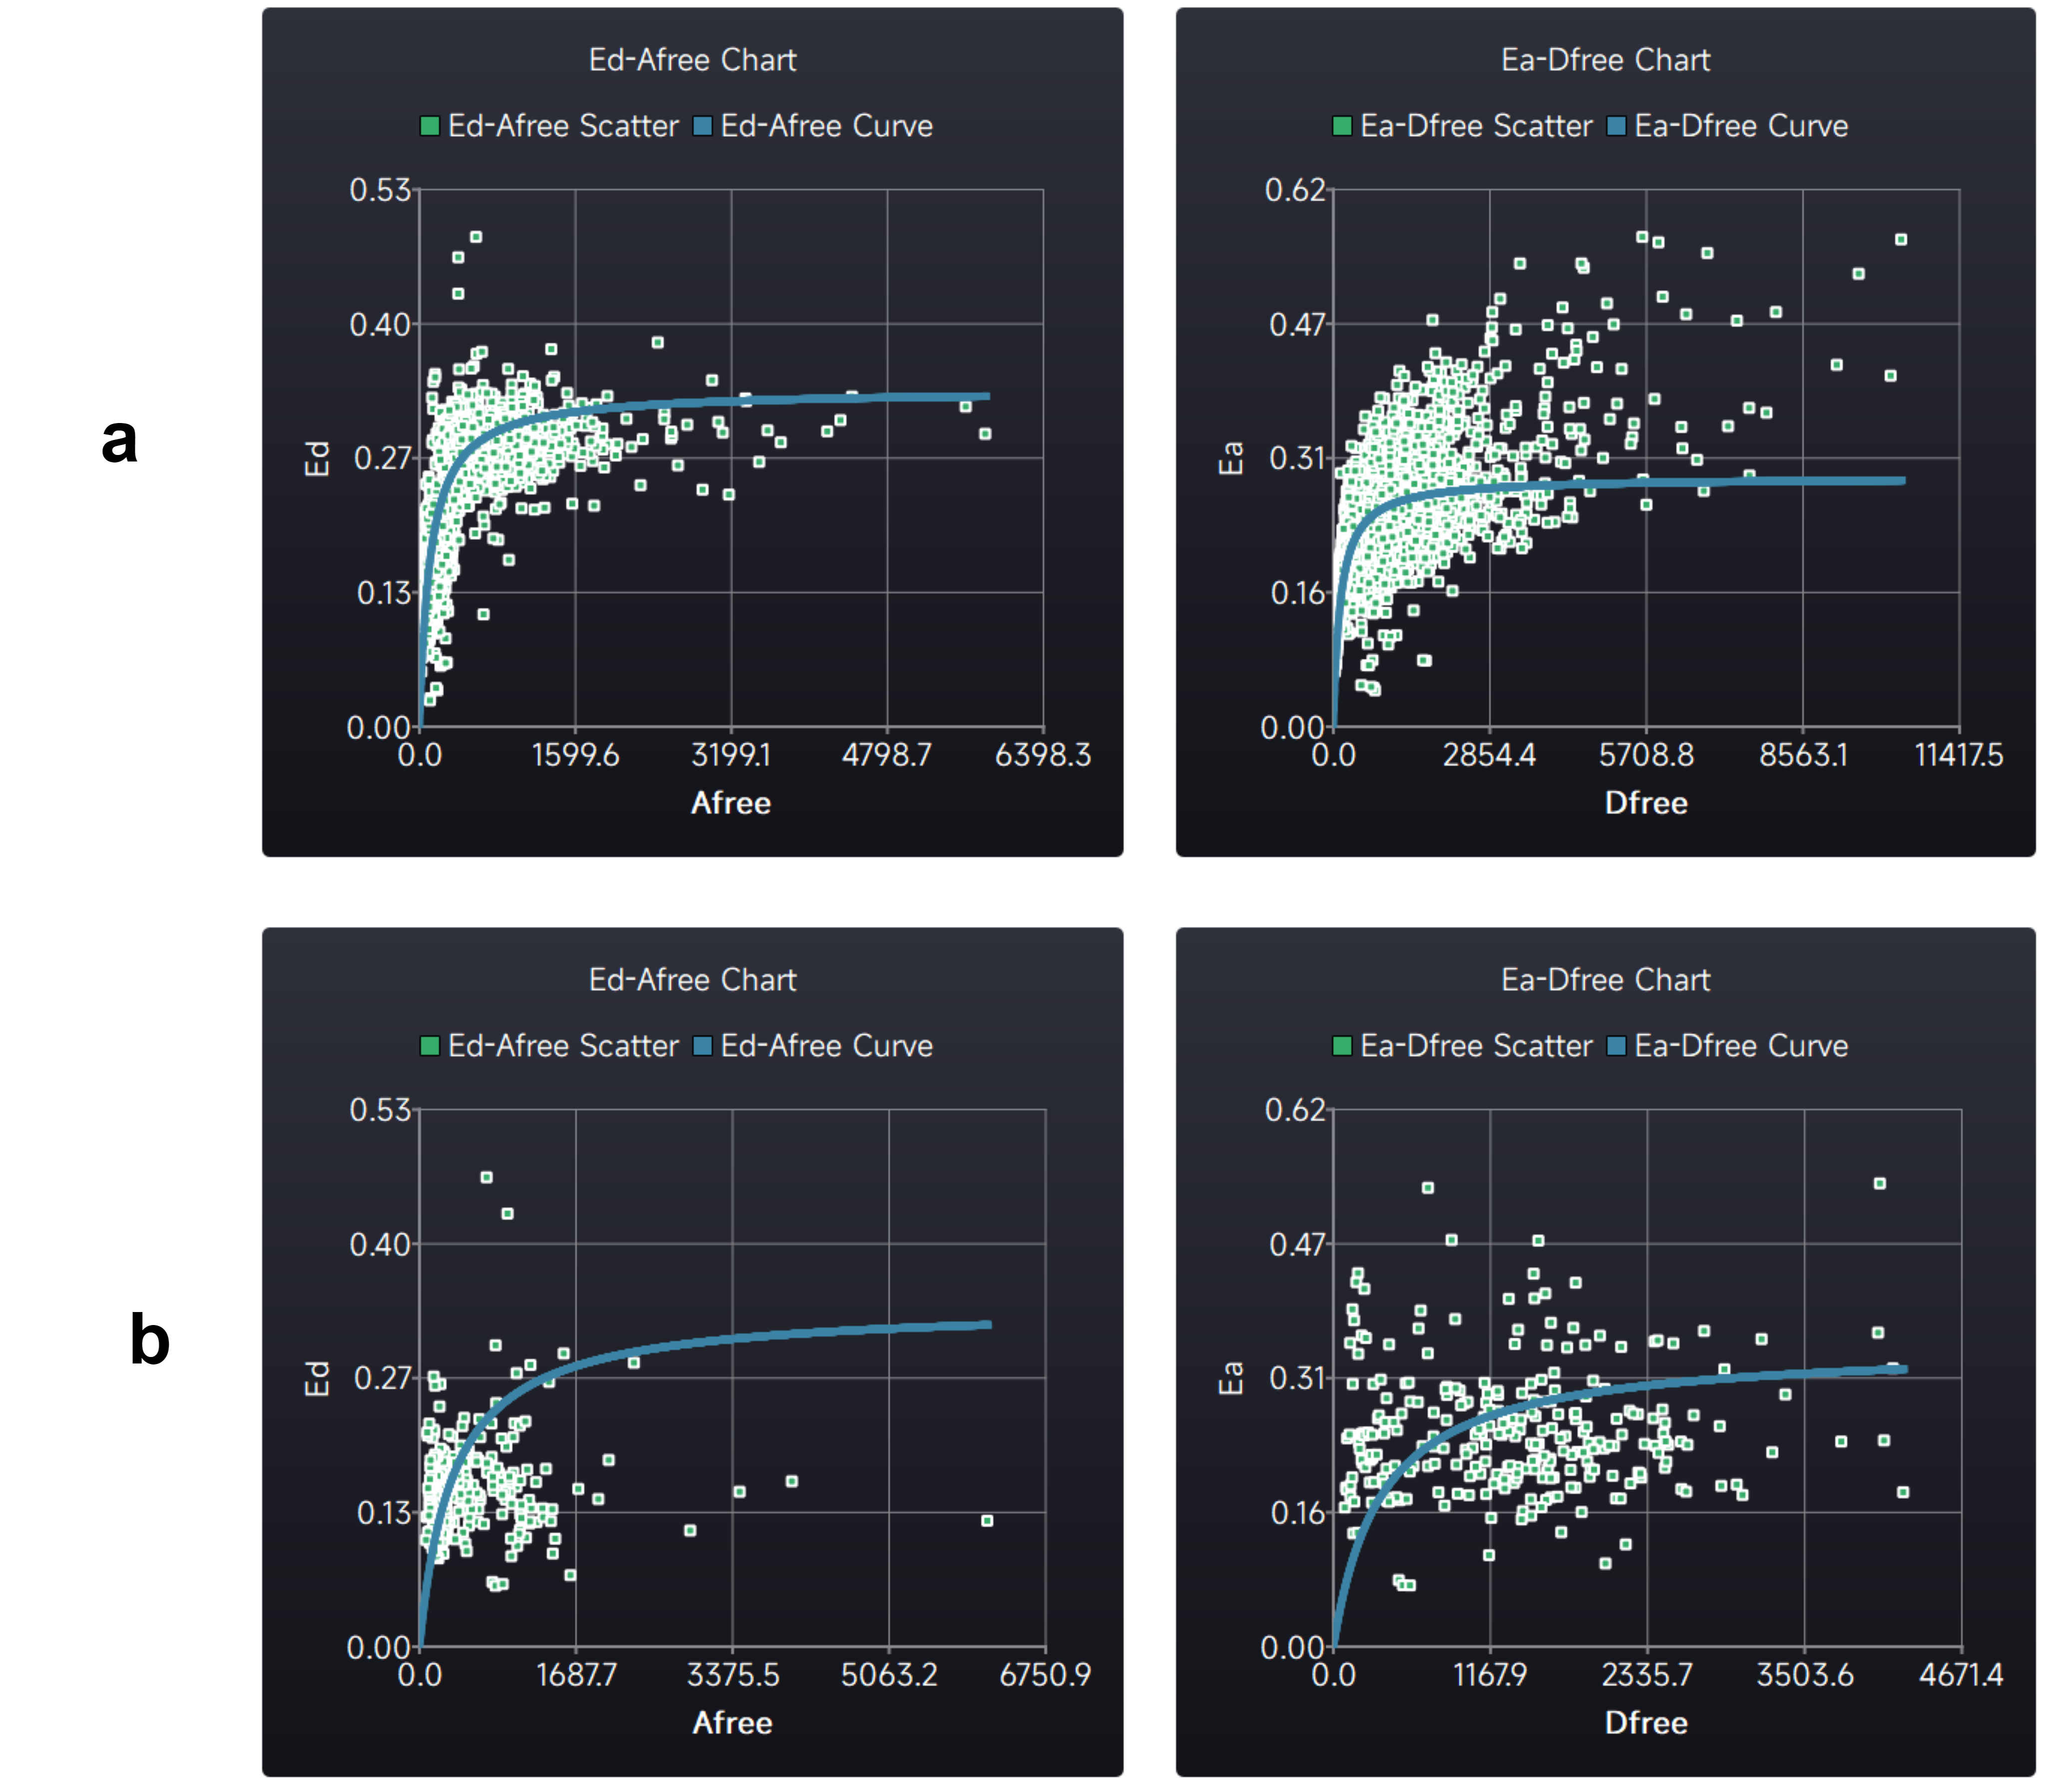
\includegraphics[width=0.9\linewidth]{../figures/4/4_L-FRET视图测试.png}
  \caption[Fretha L-FRET视图测试结果]{Fretha L-FRET视图测试结果。图a为标准L-FRET视图,图b为应用BIN数据分箱后的L-FRET视图。}
  \label{fig:L-FRET视图测试}
\end{figure}

测试DC-FRET视图中调整线性拟合的数据范围参数设置功能时,首先设置线性拟合的$R_C$数据范围为$(0,0.5)$,均值拟合的$R_C$范围为$(2,10)$,然后设置线性拟合的$1/R_C$数据范围为$(0,1)$,均值拟合的$1/R_C$范围为$(1,10)$,观察图表中的趋势线和散点图更新。
测试结果如图 \ref{fig:DC-FRET视图测试} 所示,当扩大拟合数据的范围后,可以观察到趋势线的更新,斜率拟合段和均值拟合段均延伸至$R_C$为1的位置。
\begin{figure}
  \centering
  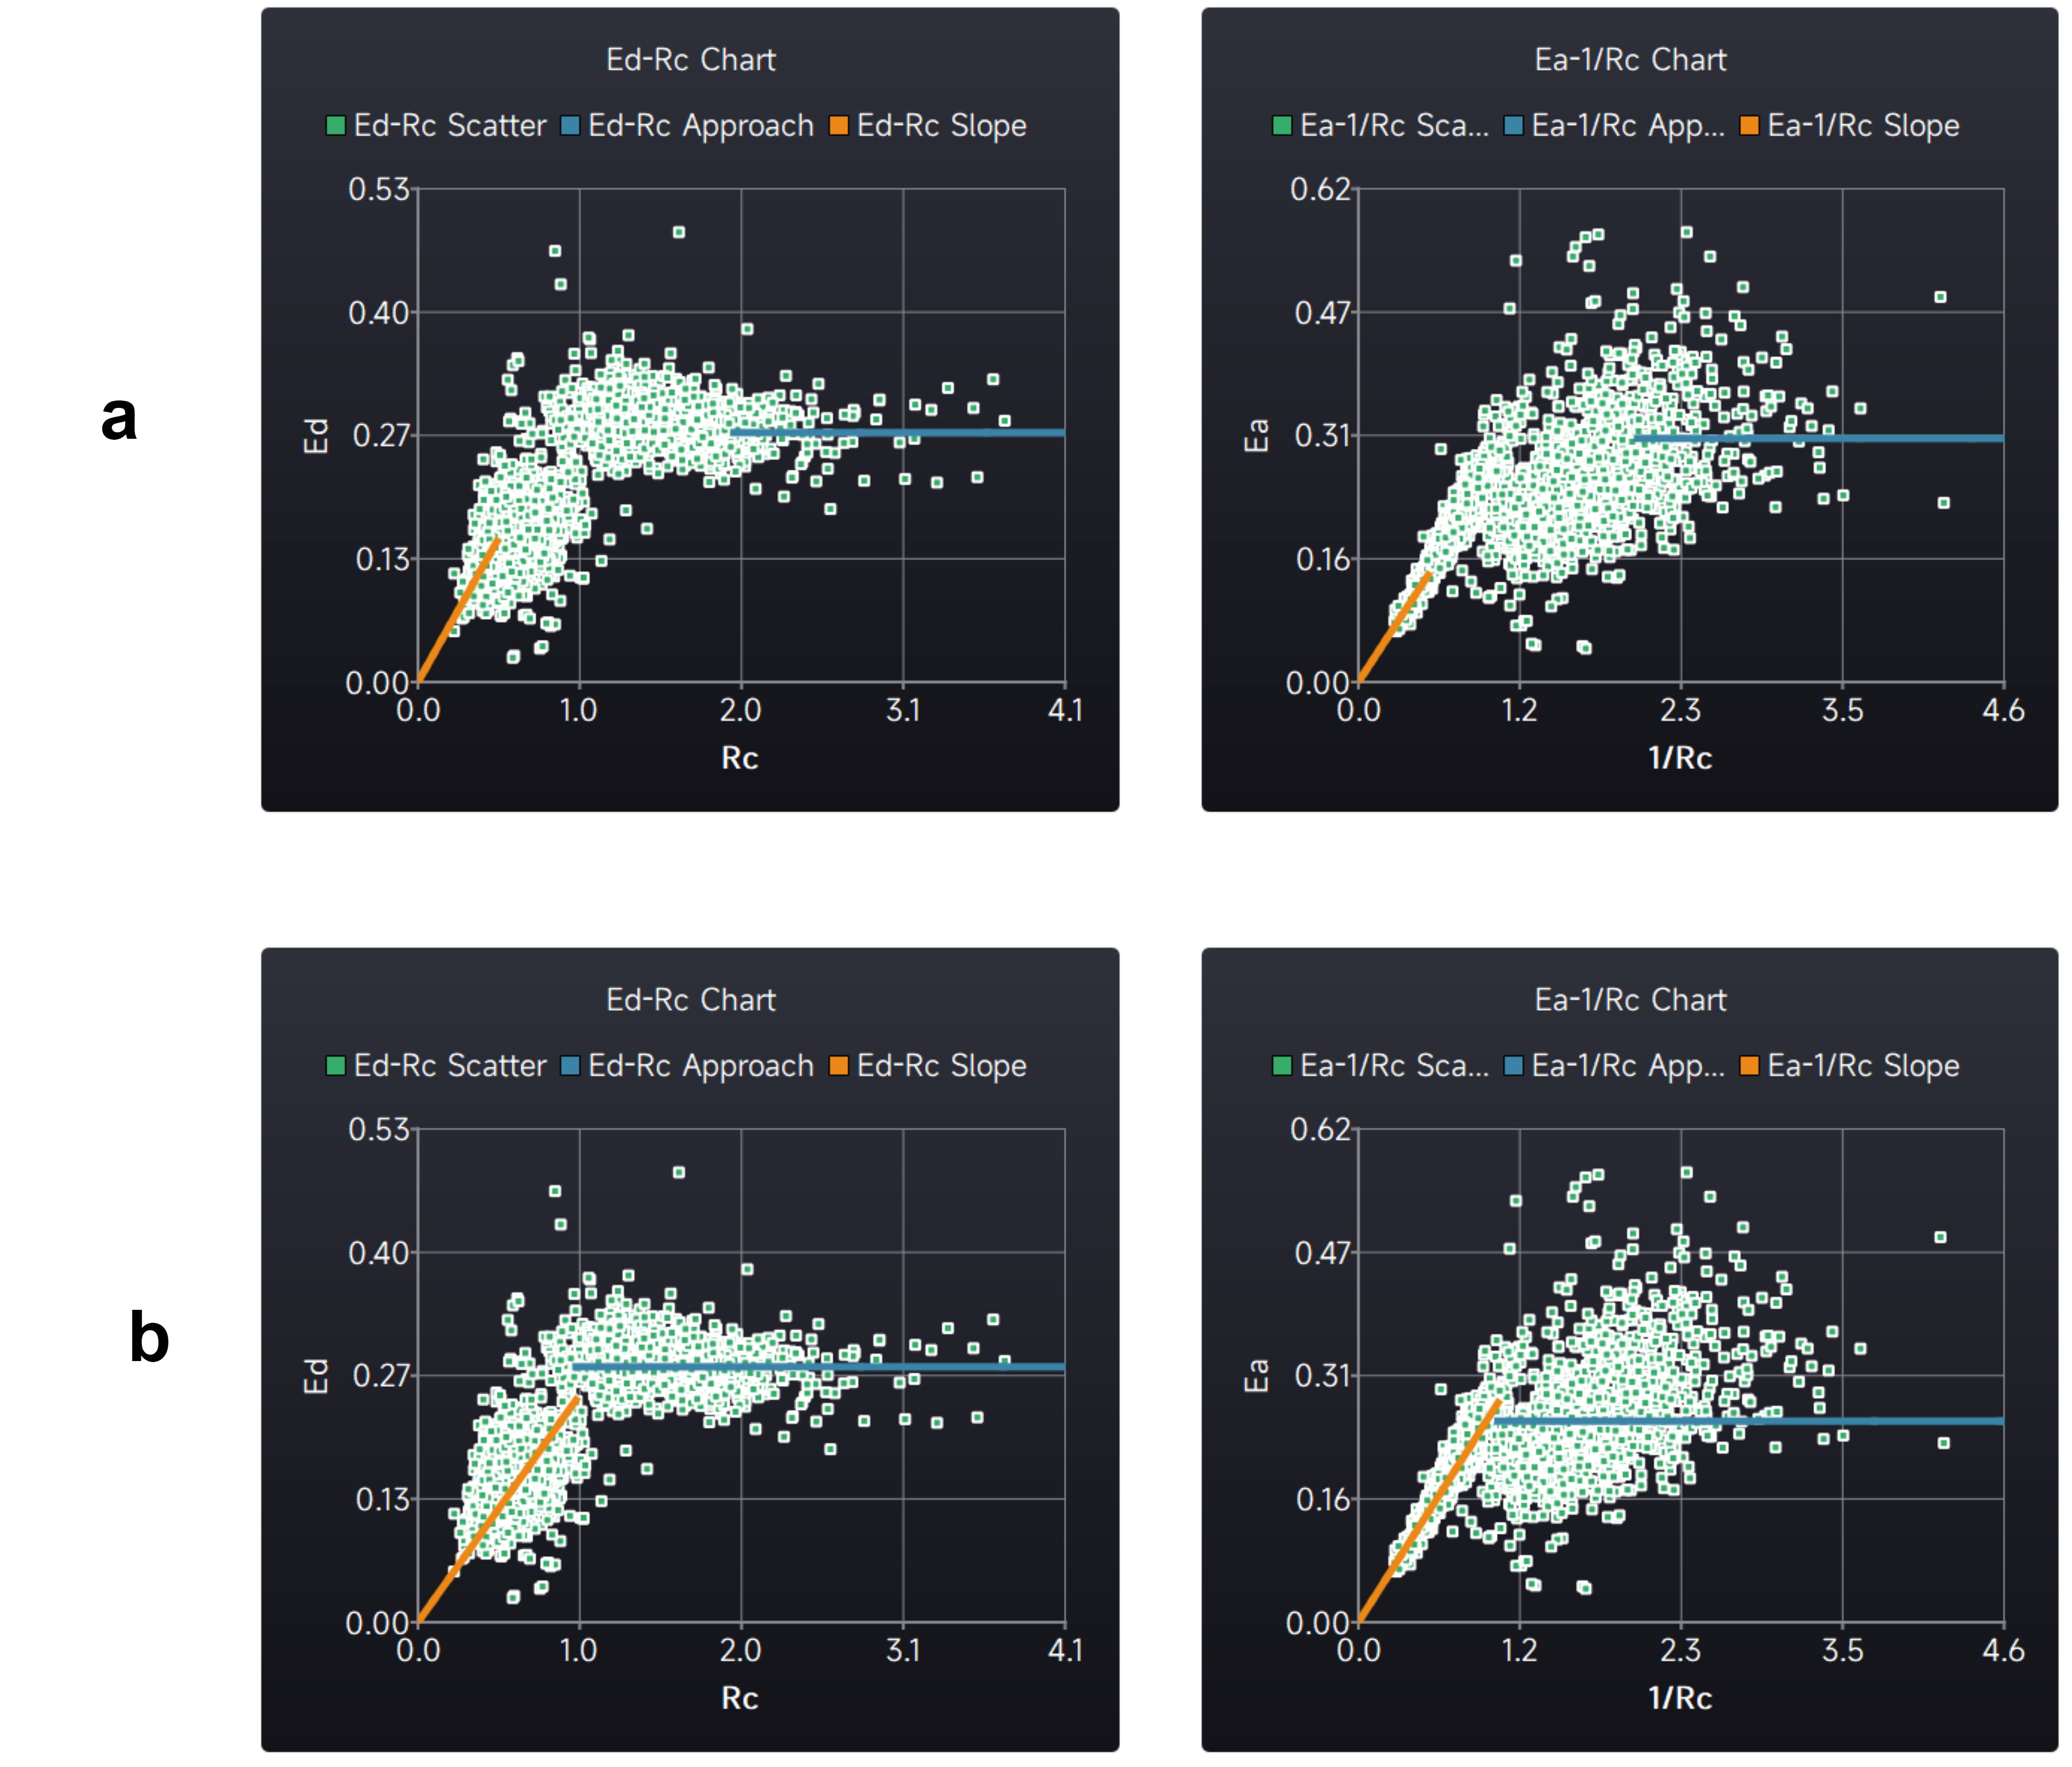
\includegraphics[width=0.9\linewidth]{../figures/4/4_DC-FRET参数测试.png}
  \caption[Fretha DC-FRET视图测试结果。]{DC-FRET视图测试结果。图a为设置线性拟合的$R_C$数据范围为$(0,0.5)$,均值拟合的$R_C$范围为$(2,10)$时Fretha生成的趋势线和散点图;
  图b则设置线性拟合的$1/R_C$数据范围为$(0,1)$,均值拟合的$1/R_C$范围为$(1,10)$。}
  \label{fig:DC-FRET视图测试}
\end{figure}

测试保存的数据和报告是否能够正确保存,结果如图 \ref{fig:结果保存测试} 所示,软件能够正确生成结果文件,且数据和报告的内容准确无误,符合预期。
\begin{figure}[hbtp]
  \centering
  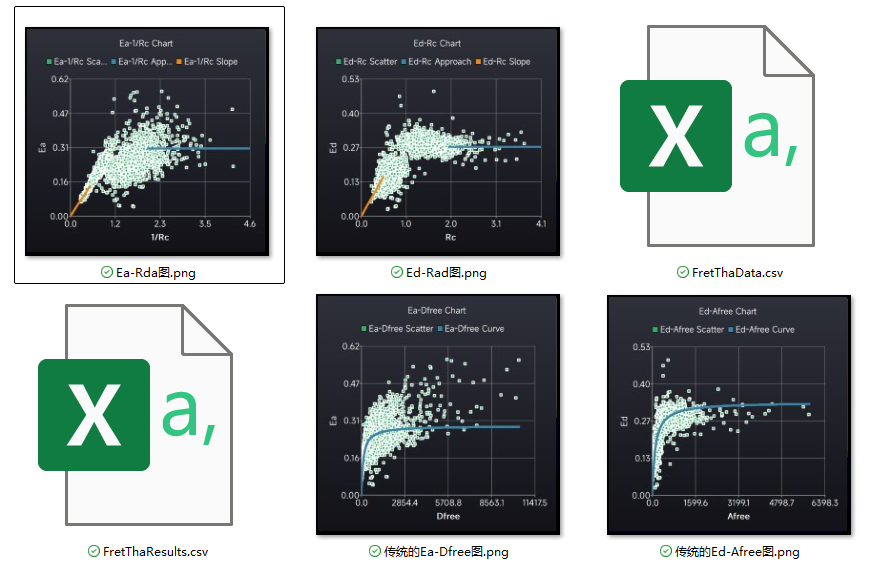
\includegraphics[width=0.6\linewidth]{../figures/2/2_保存数据.png}
  \caption{Fretha结果保存测试结果}
  \label{fig:结果保存测试}
\end{figure}

\section{自动算法性能分析}
在相同硬件配置(Intel\textsuperscript{\textregistered} Xeon E5-2678 v3 @ 2.50GHz处理器,NVIDIA\textsuperscript{\textregistered} GeForce RTX 3090 GPU)下,我们对LURS算法与两种基于深度学习的自动ROI提取方法(ilastik和SAM-Med2D)进行了系统性性能对比。

如表 \ref{tab:性能对比} 所示,LURS方法在1.4GB数据集(包含30个视野的药物处理组和对照组)中仅需20秒即可提取700个可分析信号,单ROI处理时间低至6.6 ms。
相比之下,ilastik和SAM-Med2D的单ROI处理时间分别为35.2 ms和50.7 ms,LURS的速度较ilastik提升5.3倍,较SAM-Med2D提升7.7倍。  

内存利用率方面,LURS仅占用约800 MB内存,分别为ilastik(~1.8 GB)的44\%和SAM-Med2D(~14 GB)的5.7\%。这一优化使得LURS在资源受限的环境中仍能高效运行。
此外,LURS完全依赖CPU资源,无需专用GPU加速,使其能够直接集成到实时显微镜成像系统中,为高通量筛选应用提供了硬件无关性和部署灵活性。  

上述结果表明,LURS在处理速度、内存效率和硬件适应性方面展现出显著优势。LURS算法在保证数据处理精度的同时,通过集成在Fretha软件系统中进行统一数据模型管理,优化计算流程和内存管理,显著提升了处理效率并降低了硬件依赖,为实时、高通量的FRET数据分析提供了更优的解决方案。

\begin{table*}[htbp]
    \centering
    \caption{不同算法的性能对比}
    \begin{tabular}{cccc}
    \toprule
    方法 & 单ROI处理时间(ms) & 内存占用 & 硬件依赖 \\
    \midrule
    LURS & 6.6 & ~800 MB & CPU \\
    ilastik & 35.2 & ~1.8 GB & GPU/CPU \\
    SAM-Med2D & 50.7 & ~14 GB & GPU \\
    \bottomrule
    \end{tabular}
    \label{tab:性能对比}
\end{table*}

\section{Fretha稳定性测试}
稳定性测试旨在评估 Fretha 软件在长时间运行、高负载或异常操作下的可靠性。测试方法如下:
\begin{enumerate}
  \item 压力测试:同时加载 10 个大型 FRET 数据集(每个数据集包含 50 个视野),连续执行参数设置、图像处理和结果计算操作,监测软件是否出现崩溃或内存泄漏。
  \item 长时间运行测试:保持软件连续运行 48 小时,期间定期检查各功能模块(如图像处理、数据导出)是否正常工作,记录 CPU 和内存占用情况。
  \item 异常操作测试:快速重复进行参数切换、数据导入导出、ROI 编辑等操作,模拟用户高频使用场景,观察软件的响应稳定性。
\end{enumerate}

测试结果如表格 \ref {tab:稳定性测试} 所示,Fretha 在压力测试下仍能稳定处理数据,未出现崩溃或内存溢出;长时间运行后,功能模块保持正常,资源占用无显著异常;高频操作下软件响应迅速,未出现卡顿或错误。这些结果证明 Fretha 具有良好的稳定性,能够满足科研和工业场景的长时间、高负载使用需求。

\begin{table}[htbp]
  \centering
  \caption{Fretha 软件稳定性测试结果}
  \label{tab:稳定性测试}
  \begin{tabular}{lp{5cm}p{5cm}}
  \toprule
  \textbf{测试类型}         & \textbf{测试方法}                                                                 & \textbf{测试结果}                                                                 \\
  \midrule 
  \multirow{5}{*}{压力测试} 
    & \multirow{5}{5cm}{同时加载 10 个大型 FRET 数据集(每个数据集包含 50 个视野),连续执行参数设置、图像处理和结果计算操作,监测软件是否出现崩溃或内存泄漏。} 
    & - 处理 10 个数据集总耗时:42.5 分钟 \\
    &                                                                                
    & - 内存峰值占用:1.4 GB(稳定无泄漏) \\
    &                                                                                
    & - 操作成功率:100\% \\
  \midrule % 测试类型分隔线
  \multirow{5}{*}{长时间运行测试} 
    & \multirow{5}{5cm}{保持软件连续运行 48 小时,期间定期检查各功能模块(如图像处理、数据导出)是否正常工作,记录 CPU 和内存占用情况。} 
    & - CPU 平均使用率:22-25\%(波动<3\%) \\
    &                                                                                
    & - 内存平均占用:550-600 MB(无持续增长) \\
    &                                                                                
    & - 数据导出成功率:100\% \\
  \midrule % 测试类型分隔线
  \multirow{4}{*}{异常操作测试} 
    & \multirow{4}{5cm}{快速重复进行参数切换、数据导入导出、ROI 编辑等操作,模拟用户高频使用场景,观察软件的响应稳定性。} 
    & - 每秒操作次数:15-20 次/秒 \\
    &                                                                                
    & - 平均响应时间:0.3-0.5 秒 \\
    &                                                                                
    & - 未出现卡顿或界面冻结 \\
    \\
  \bottomrule
  \end{tabular}
\end{table}

\section{本章小结}

本章对Fretha软件的各功能模块进行了全面的测试与验证,包括成像参数设置模块、数据检验模块、FRET图像处理模块、数据管理模块、结果可视化模块以及自动算法性能和软件稳定性测试。
测试结果表明,Fretha软件在功能实现、性能表现和稳定性方面均达到了预期目标。成像参数设置模块能够准确更新和保存参数,确保了数据处理的可靠性;
数据检验模块有效识别并隔离异常数据,保障了数据完整性和计算安全性;
FRET图像处理模块在视图增强、ROI编辑和状态栏更新等功能上表现出色,显著提升了用户操作的便捷性和精确性;数据管理模块支持多种数据操作,功能完善且运行稳定;
结果可视化模块能够直观展示分析结果,支持多种视图切换和参数调整,满足了用户对结果展示的多样化需求。
此外,LURS算法在处理速度、内存效率和硬件适应性方面展现出显著优势,为高通量实时分析提供了高效的解决方案。
稳定性测试进一步验证了Fretha在长时间运行、高负载和高频操作下的可靠性,未出现崩溃或性能下降的情况。
综合测试结果表明,Fretha软件功能完善、性能优越、稳定性良好,能够满足复杂科研和实际应用的需求。